\subsection{Optical Flow}
\begin{frame}{Measuring Motion: Optical Flow}
    \begin{itemize}
        \item Computes a dense motion field between consecutive frames.
        \item Popular algorithms:
        \begin{itemize}
            \item Farneback
            \item TV-L1
        \end{itemize}
        \item Optical flow is commonly used as input to Two-Stream Networks for action recognition.
    \end{itemize}
\end{frame}

\begin{frame}[allowframebreaks]{Optical Flow: Key Concepts}
    \begin{itemize}
        \item \textbf{Dense Motion Field}: Represents motion vectors for every pixel between two frames.
        \item \textbf{Temporal Coherence}: Assumes that motion is smooth and continuous over time.
        \item \textbf{Applications}: Used in action recognition, video segmentation, and object tracking.
    \end{itemize}
\framebreak
    \begin{figure}
        \centering
        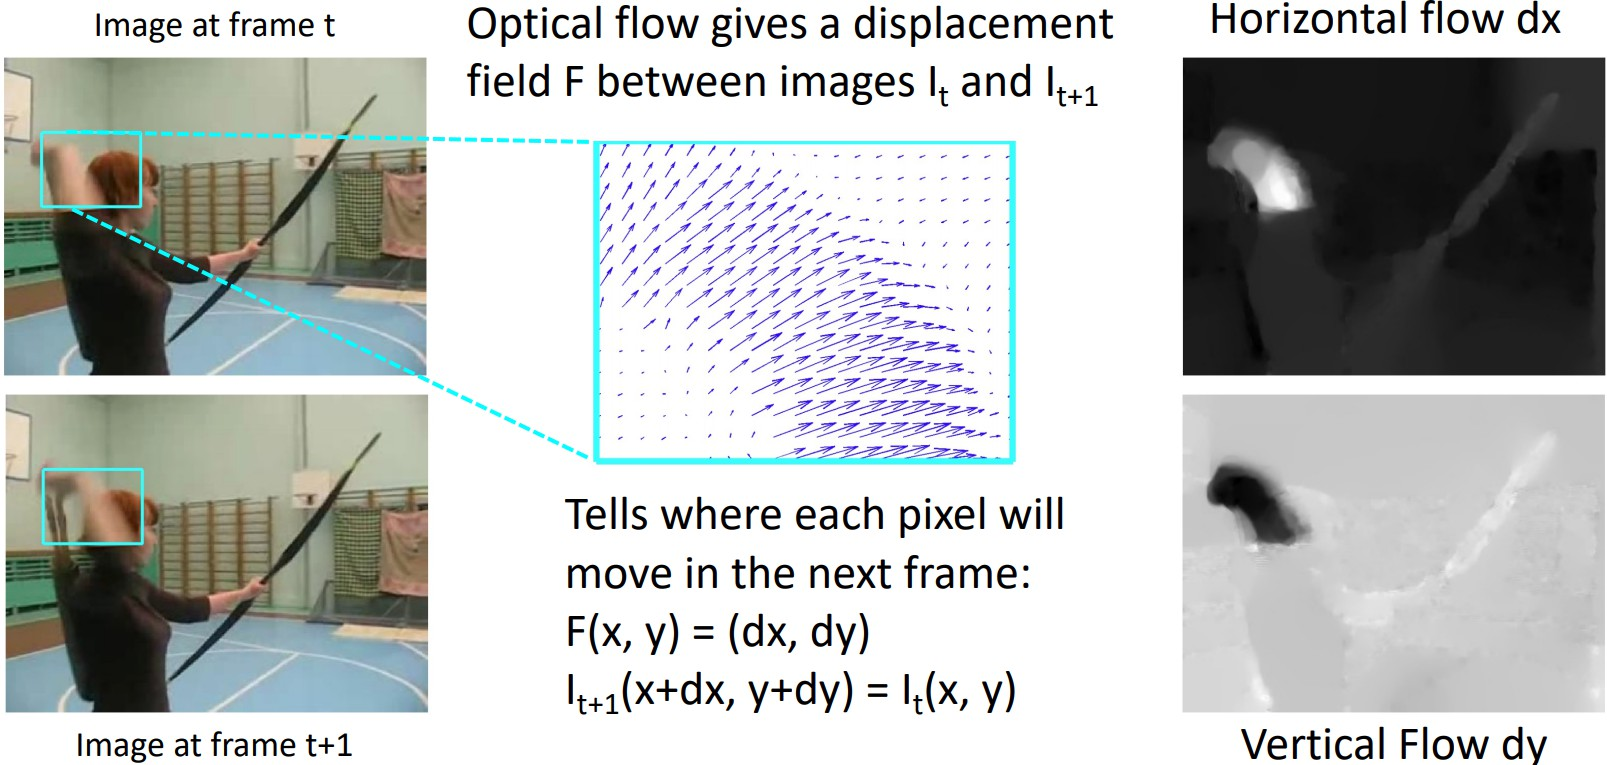
\includegraphics[width=1\textwidth,height=0.9\textheight,keepaspectratio]{images/video/slide_22_1_img.jpg}
    \end{figure}
\end{frame}